\documentclass[11pt,a4paper]{article}
	\usepackage[T2A]{fontenc}
	\usepackage[english]{babel}
	\usepackage{indentfirst}
	\usepackage{tipa}
	\usepackage{graphicx}
	\usepackage{hyperref}
	\usepackage{afterpage}
%	\usepackage{}
%	\usepackage[usestackEOL]{stackengine}
%	\makesavenoteenv{tabular}
	\usepackage[
    	type={CC},
    	modifier={by-nc},
    	version={4.0},
	]{doclicense}
%	\usepackage{cclicenses}
	\graphicspath{{images/}}
	\title{\textbf{The Fomenkos Ukrainian cuisine family cookbook}}
	\author{Oleksii Fomenko}
	\date{}

	\addtolength{\topmargin}{-2cm}
	\addtolength{\textheight}{2cm}
	
\begin{document}

\section*{Disclaimer}
These recipes are not 'canonical' ones, just like my wife and myself are cooking every day so please add 'in our family' for the every recipe here.
\\

Note: mostly Ukrainian meals are not halal or kosher due to massive pork, lard and meat+milk usage but I'll try to modify recipes or write an alternative ways to cook for non-Ukrainians. I'll really try, I swear :-)
\\
\\
All photos are made by myself using ordinary smartphone, maybe some day I will ask somebody to use good camera for these recipes.
\\
%\cc \bync

\section*{Борщ Borshch \textipa{['bO:rS]}}
Maybe the very first everyone is remaining when hearing anything about 'Ukrainian cuisine'.
Yes, that's the most popular and most controversial meal. It has the only necessary ingredient -- beetroot (but not always, 'Green Borshch' has no beetroot at all but sorrel or even spinach instead).

\subsection*{Ordinary Borshch}
All borshchs traditionally made using pork broth but chicken or even mushroom or vegetable ones are used as well (Eastern Christians has four periods a year when they cannot eat any meat. I'm an atheist but who can stop me to use alternative ingredients?)

In this recipe I'm using 6-liter pot. \\

Ingridients:
\begin{itemize}
\item One chicken
\item Beetroot
\item Cabbage
\item Carrot
\item Potatoes
\item Onions
\item Tomato paste or fresh tomatoes
\item Greens
\item Red beans
\item Lard (\textbf{not kosher or halal!}) or frying oil (does not matter, sunflower, olive or any else)
\item Optional: beetroot juice
\item Optional: sour cream or plain yoghurt (\textbf{not kosher!})
\end{itemize}

Take one chicken. I'm using farmer's chicken here (the older is better):
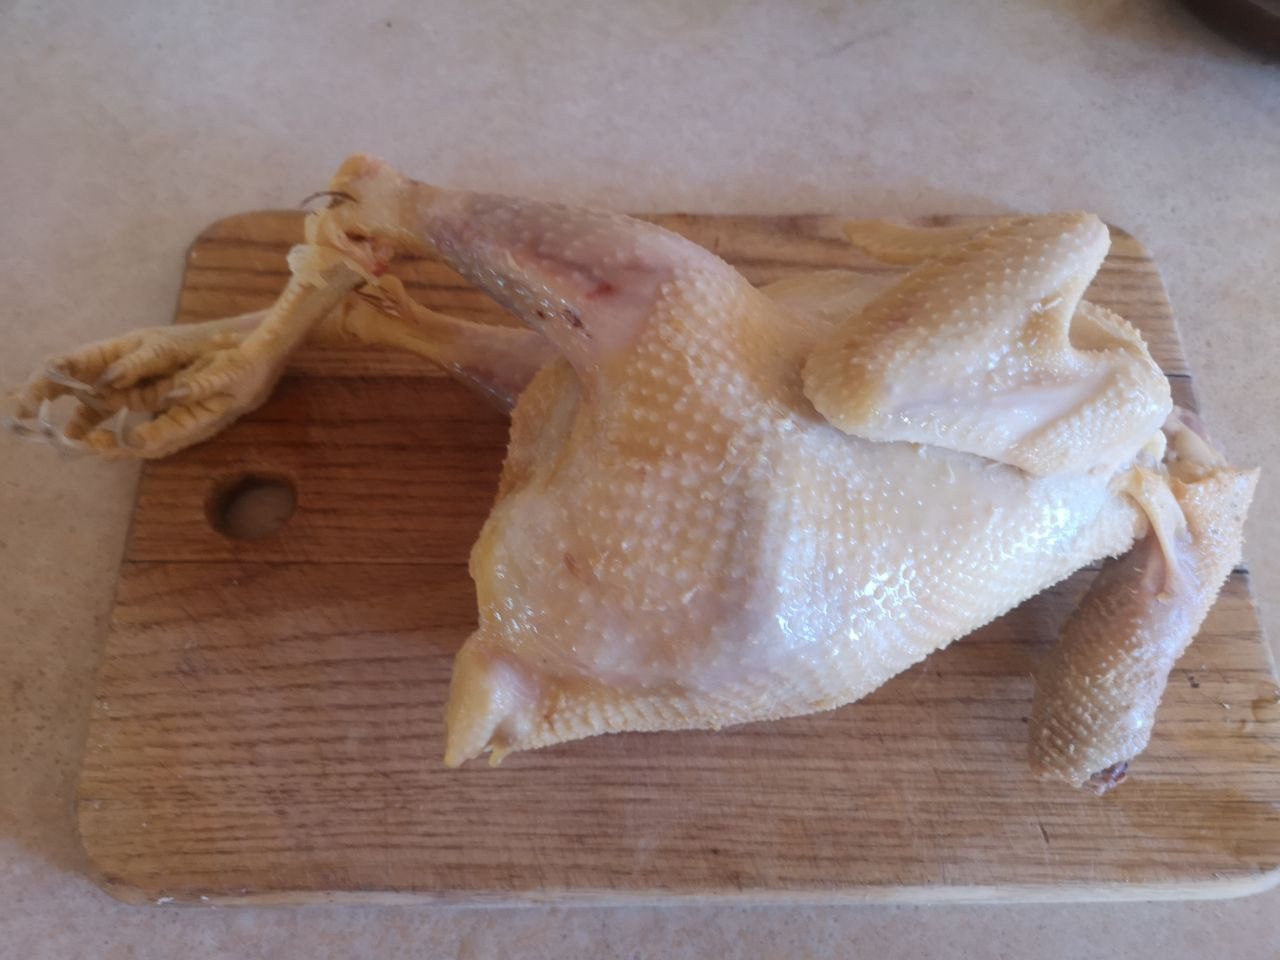
\includegraphics[width=\textwidth]{1.jpg}

Remove all excess (remains of feathers, talons etc.), put it in the pot, add about 3 liters of water, boil quickly and set the minimum possible temperature when boiled. Leave it on three hours and don't forget to remove froth. Optionally you can add there some parsley root, celery root, onion, carrot and bay leafs; 'cage' like this is very useful (anyway all roots and vegetables boiled during this time must be removed when ready):\\

\includegraphics[width=\textwidth]{2.jpg}
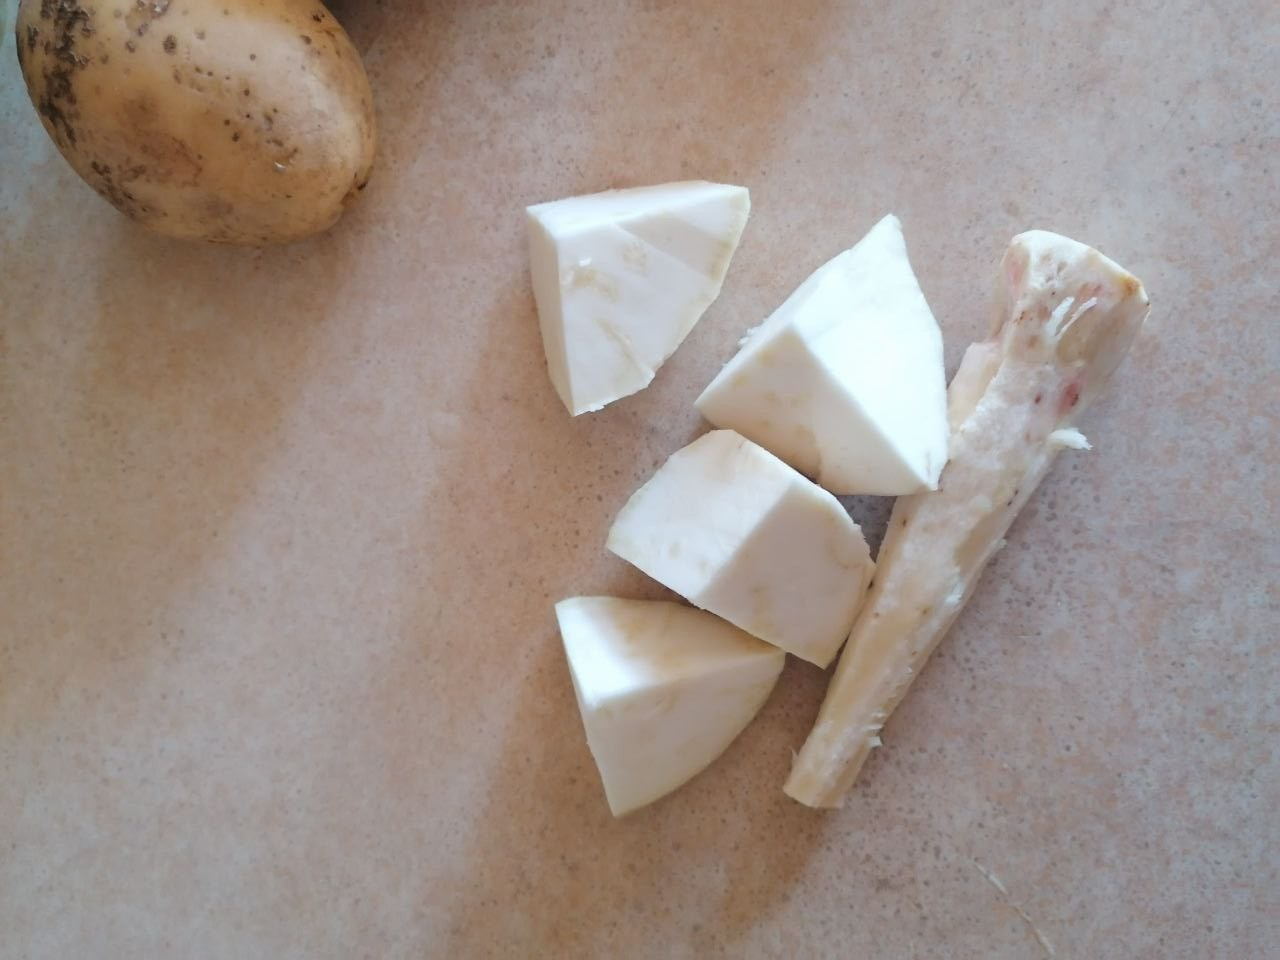
\includegraphics[width=\textwidth]{4.jpg} \\


While our chicken is boiling let's prepare other ingredients:\\
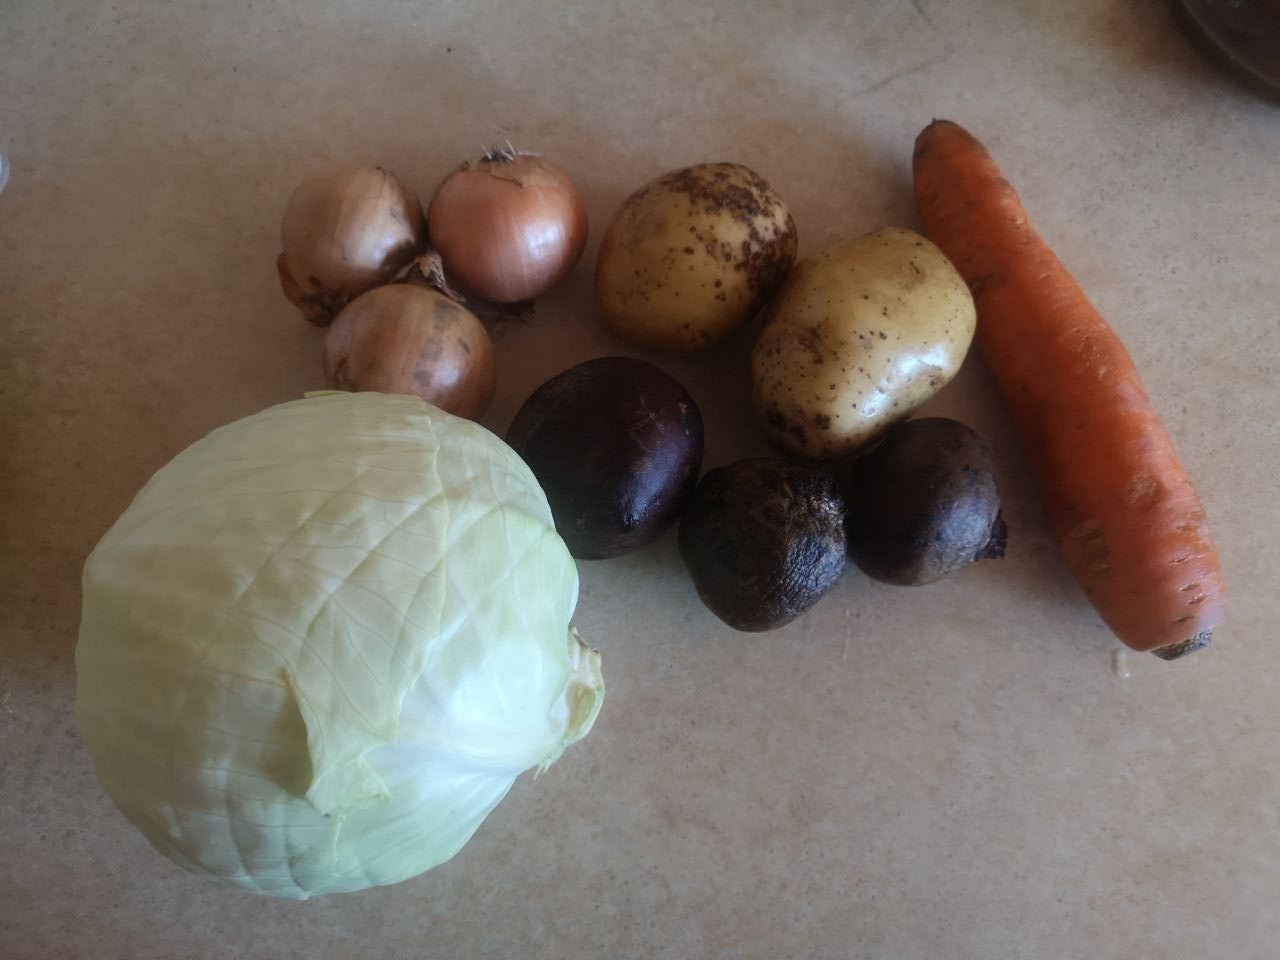
\includegraphics[width=\textwidth]{3.jpg}

Note: botshch is mostly beetroot, not cabbage meal so we don't need a lot of cabbage there. \\

Slice 1/4 of cabbage and put aside: \\
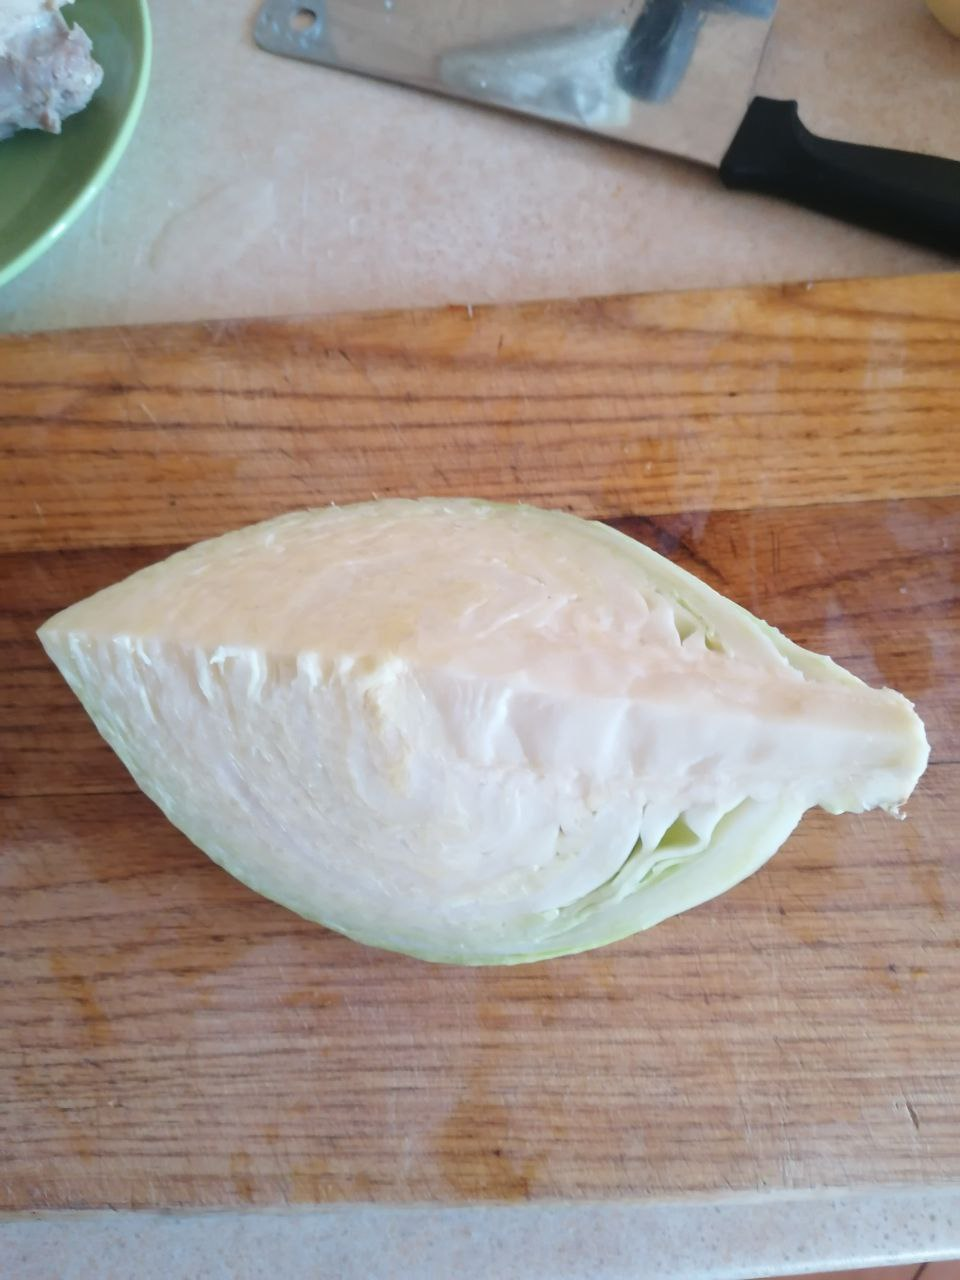
\includegraphics[width=\textwidth]{5.jpg}
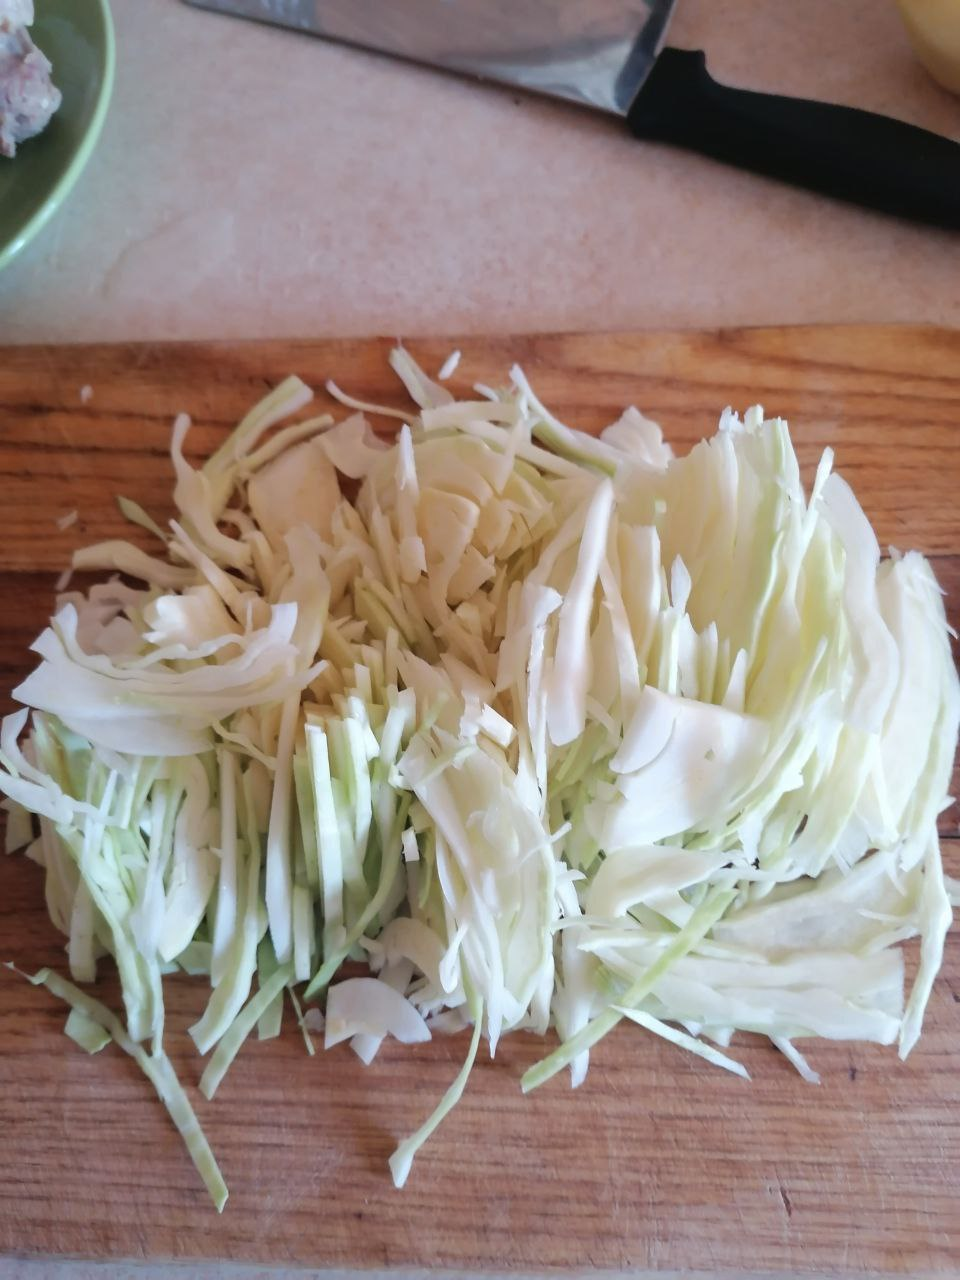
\includegraphics[width=\textwidth]{6.jpg} \\

Slice onions and add them to sliced cabbage: \\
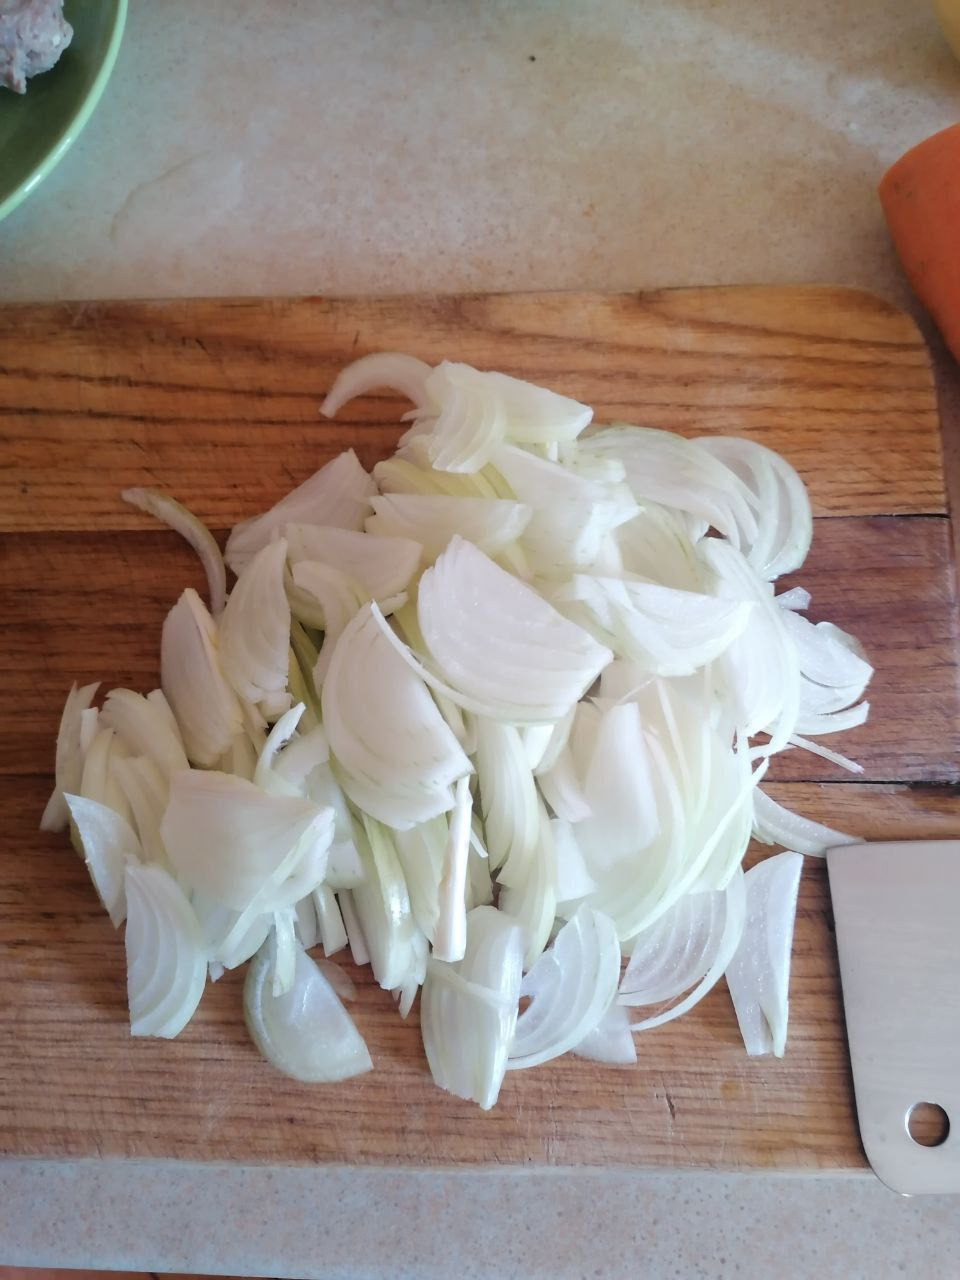
\includegraphics[width=\textwidth]{7.jpg} \\

Grind carrot and beetroot, add them to cabbage and onions: \\
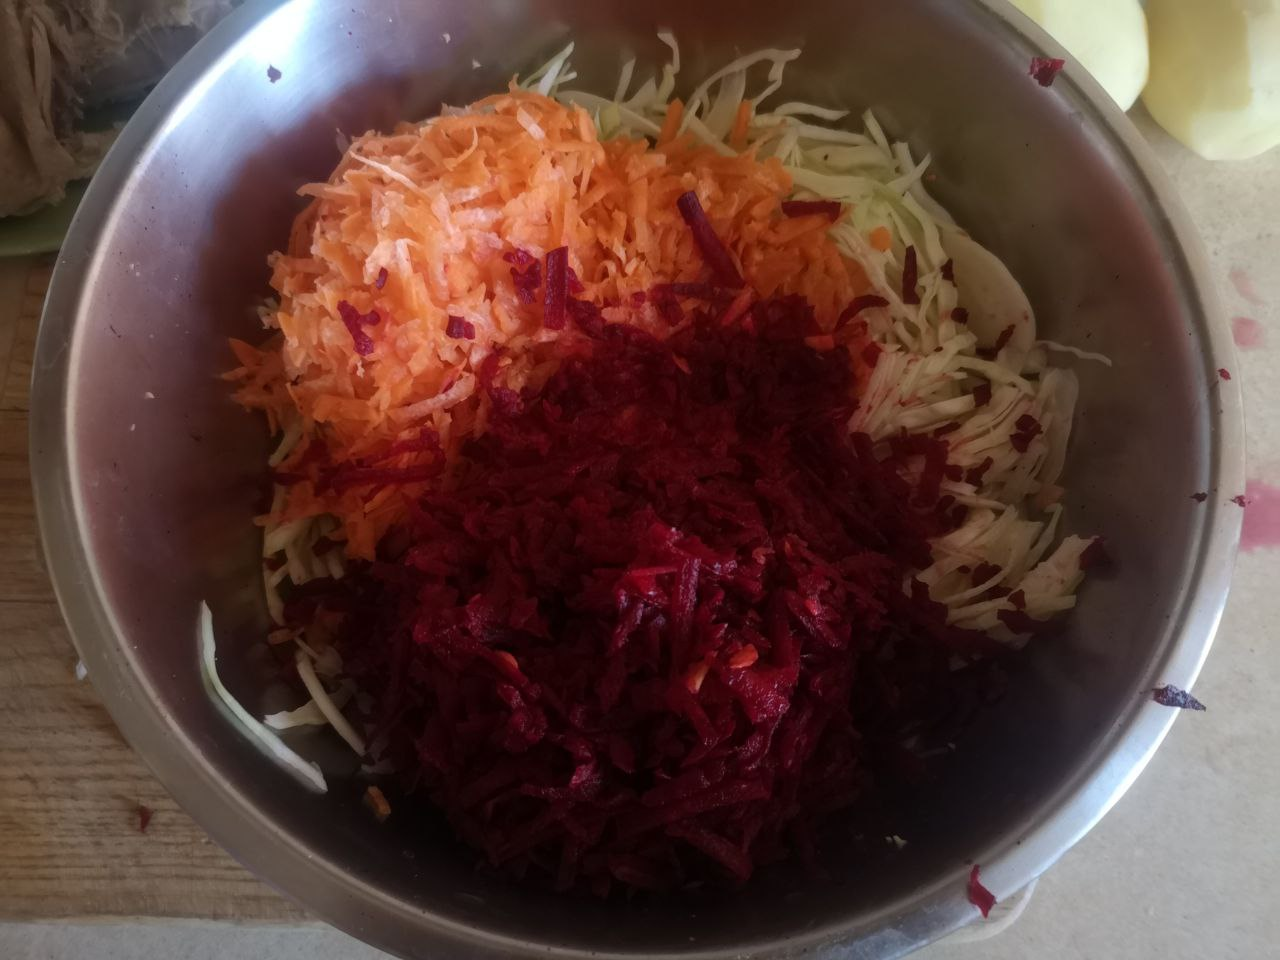
\includegraphics[width=\textwidth]{8.jpg} \\

Take a big frying pan, add there some lard or oil and stir fry sliced and ground vegetables: \\
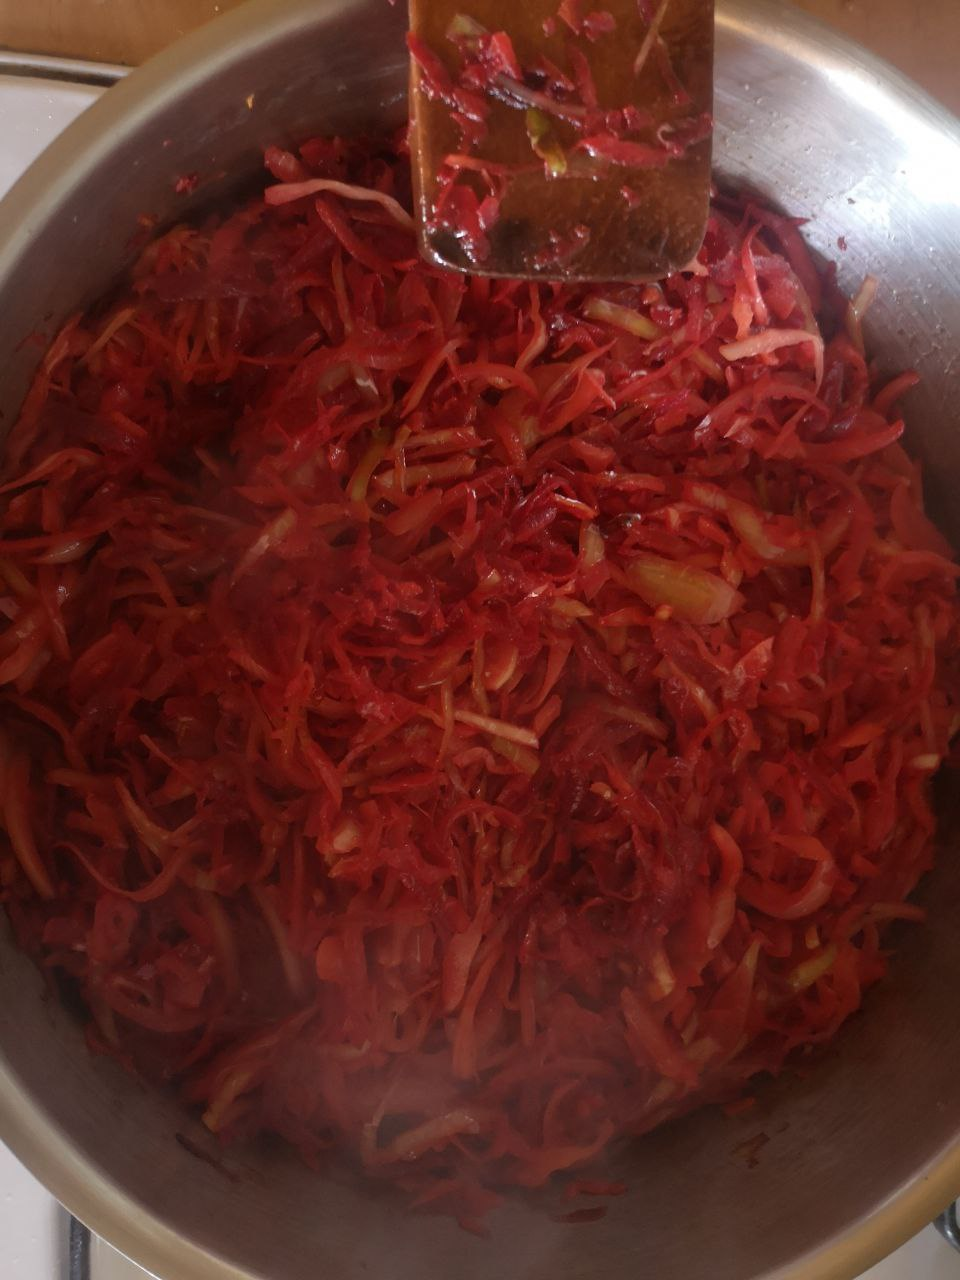
\includegraphics[width=\textwidth]{9.jpg} \\
Add one spoonful of vinegar when vegetables became soft, it returns bright color. Add tomato paste (or diced tomatoes without skin): \\
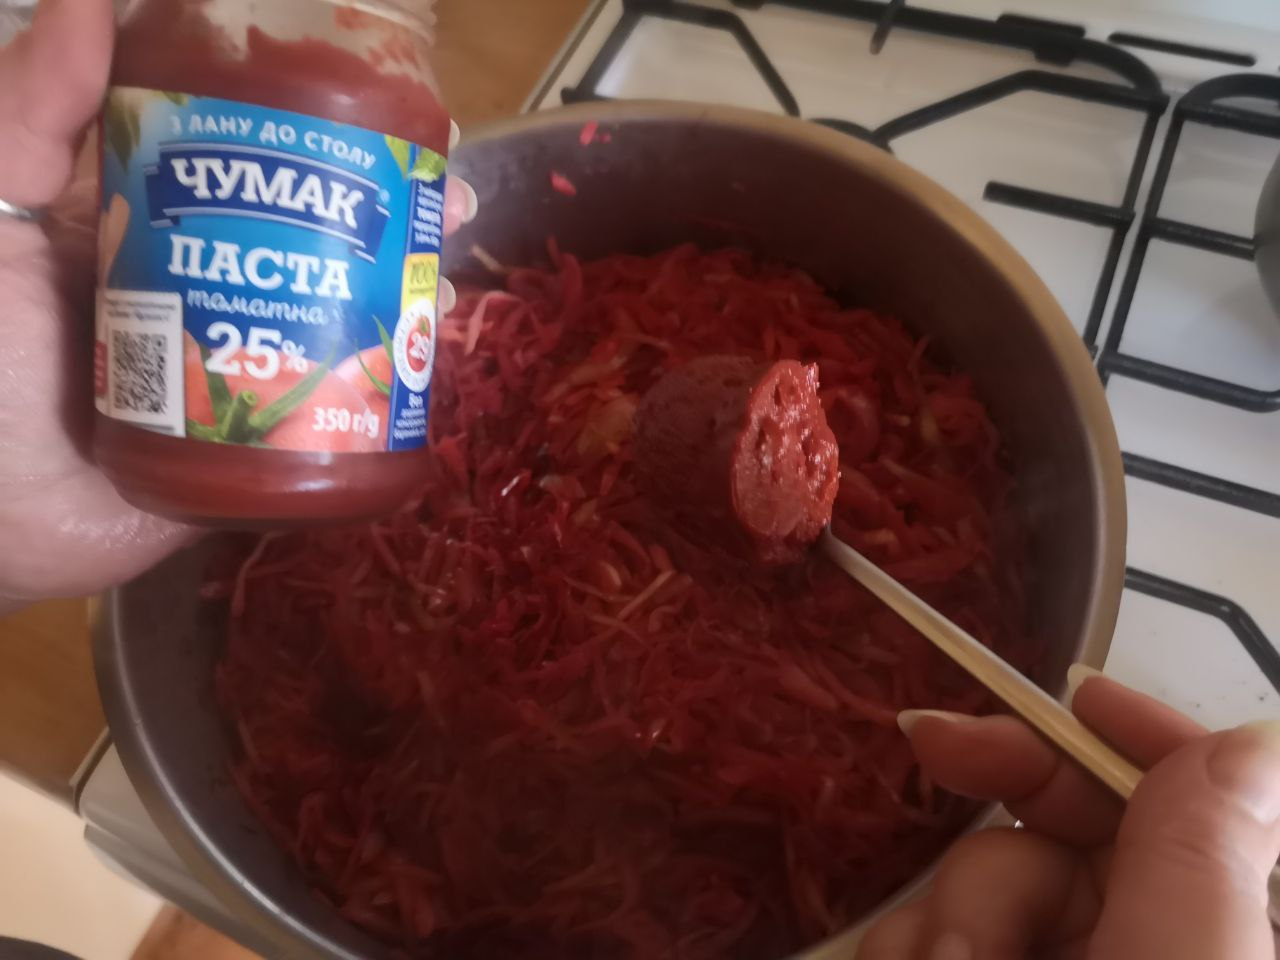
\includegraphics[width=\textwidth]{10.jpg} \\

Dice potatoes: \\
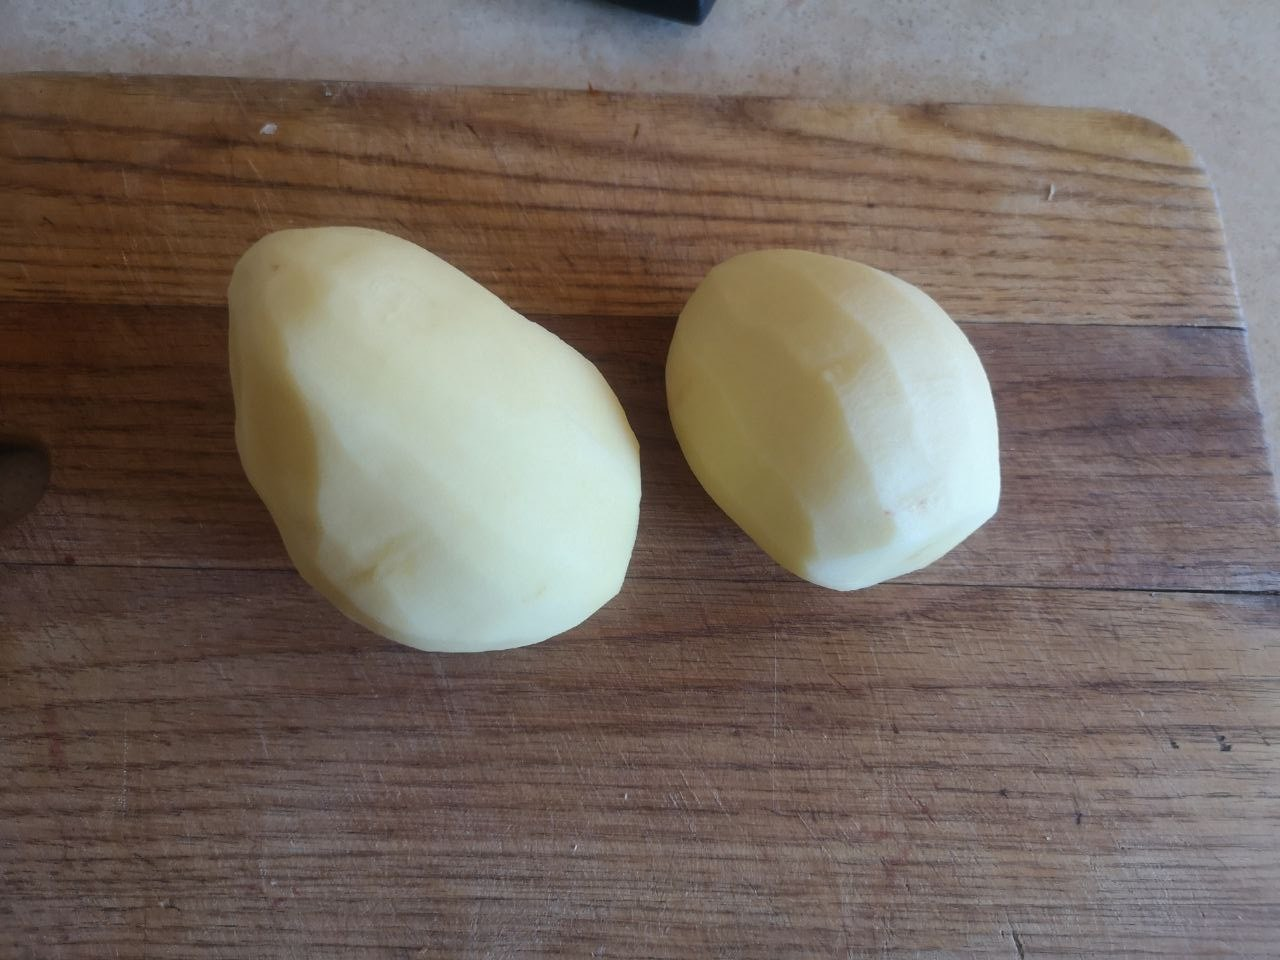
\includegraphics[width=\textwidth]{11.jpg} \\
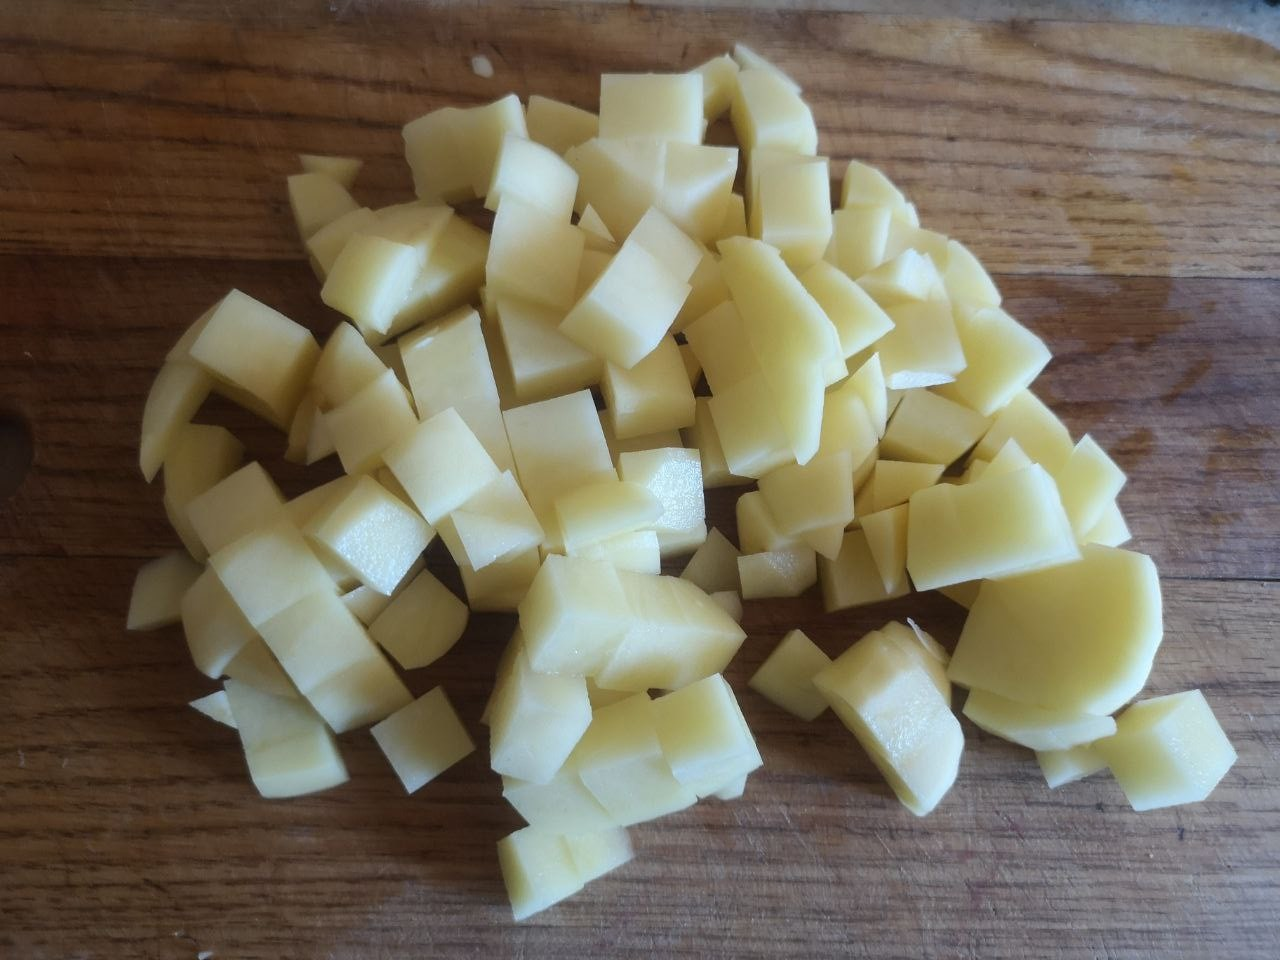
\includegraphics[width=\textwidth]{12.jpg} \\

Remove chicken and roots from pot and put there fried vegetables. Remove meat from chicken and dice it: \\
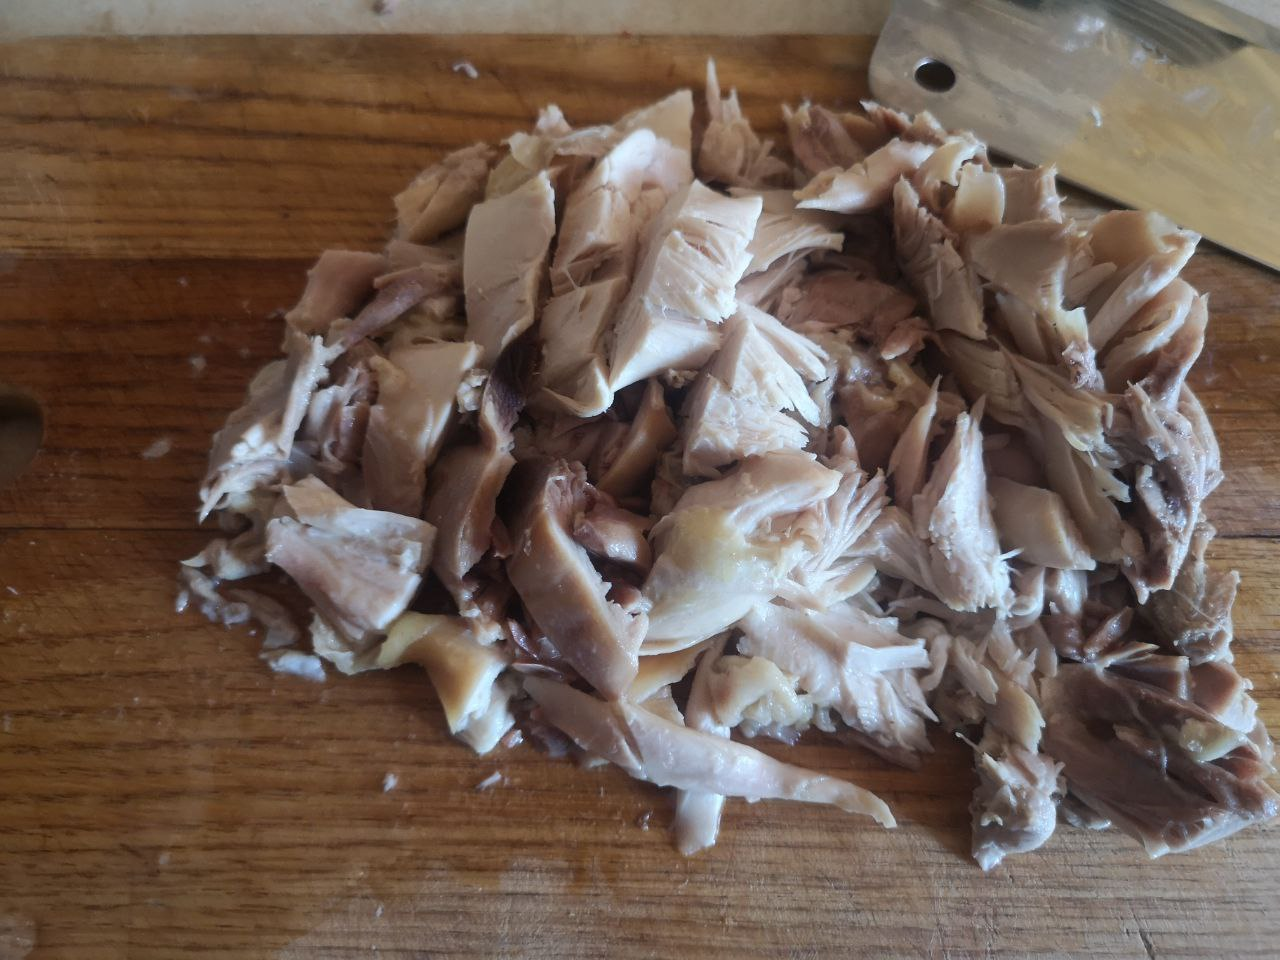
\includegraphics[width=\textwidth]{13.jpg} \\

Add red beans to the pot (I'm using canned ones but you can soak them overnight before cooking and add then): \\
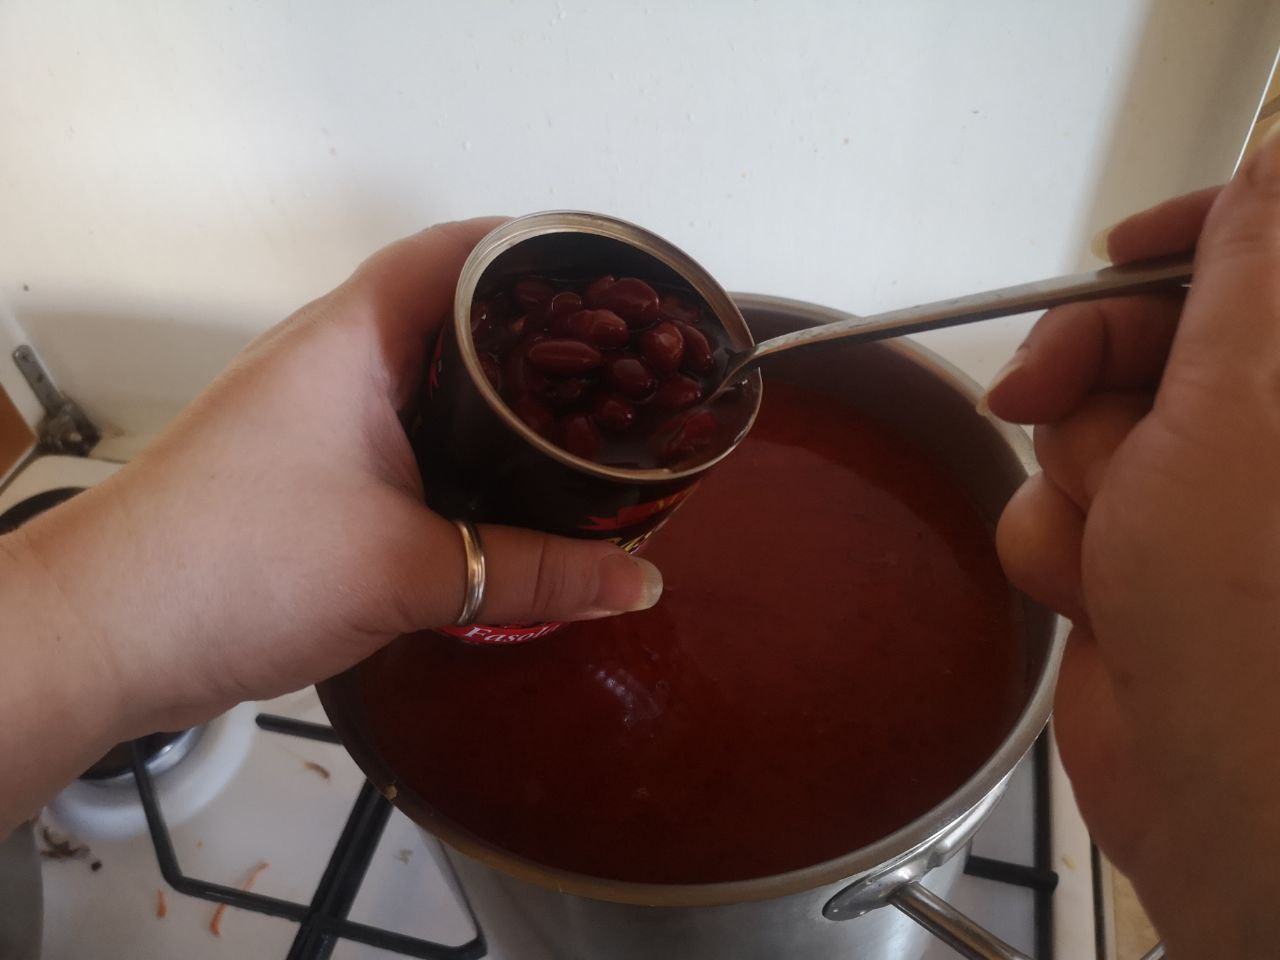
\includegraphics[width=\textwidth]{14.jpg} \\

If you have Polish grocery nearby you can buy beetroot juice (or concentrate) and add it to the pot, they call it 'Barszczyk Czerwony' (photo from https://rolnik.pl): \\
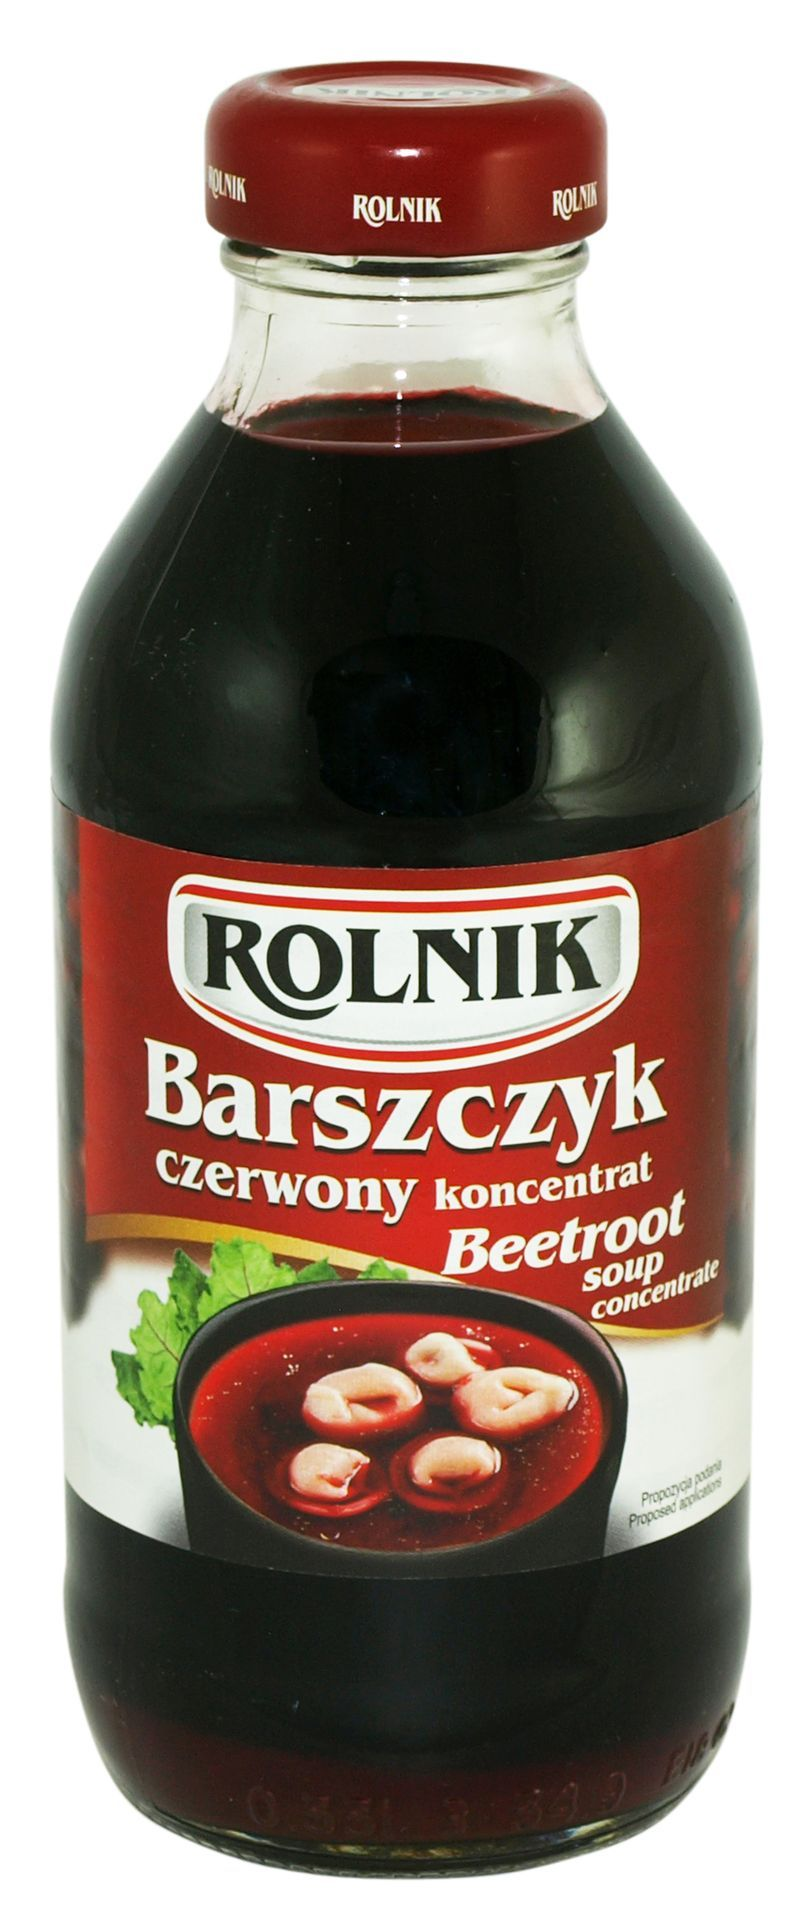
\includegraphics{15.jpg} \\

Dice dill, parsley and garlic (if you have no fresh ones at the moment you can use dried): \\
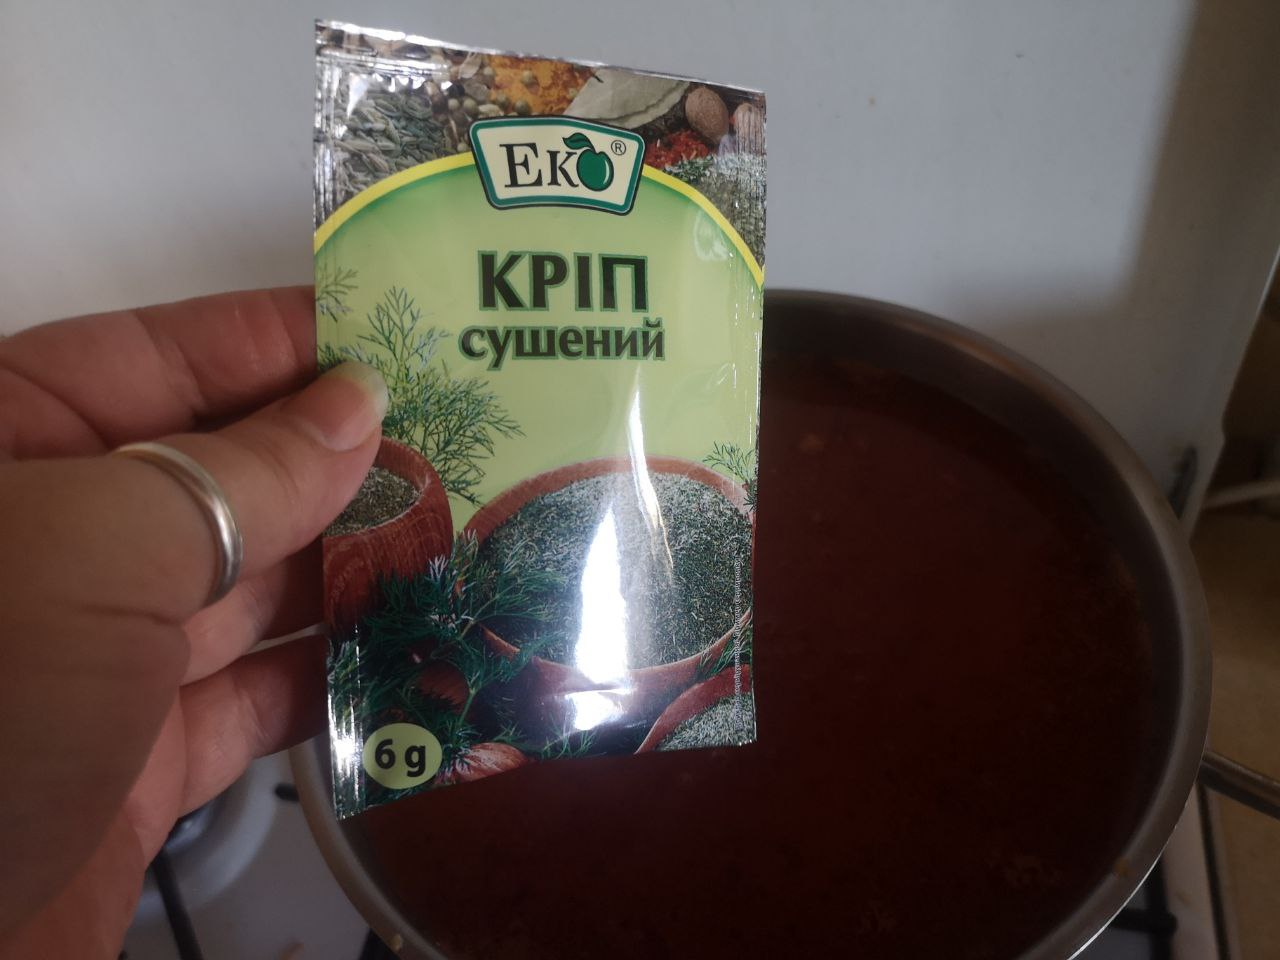
\includegraphics[width=\textwidth]{16.jpg} \\
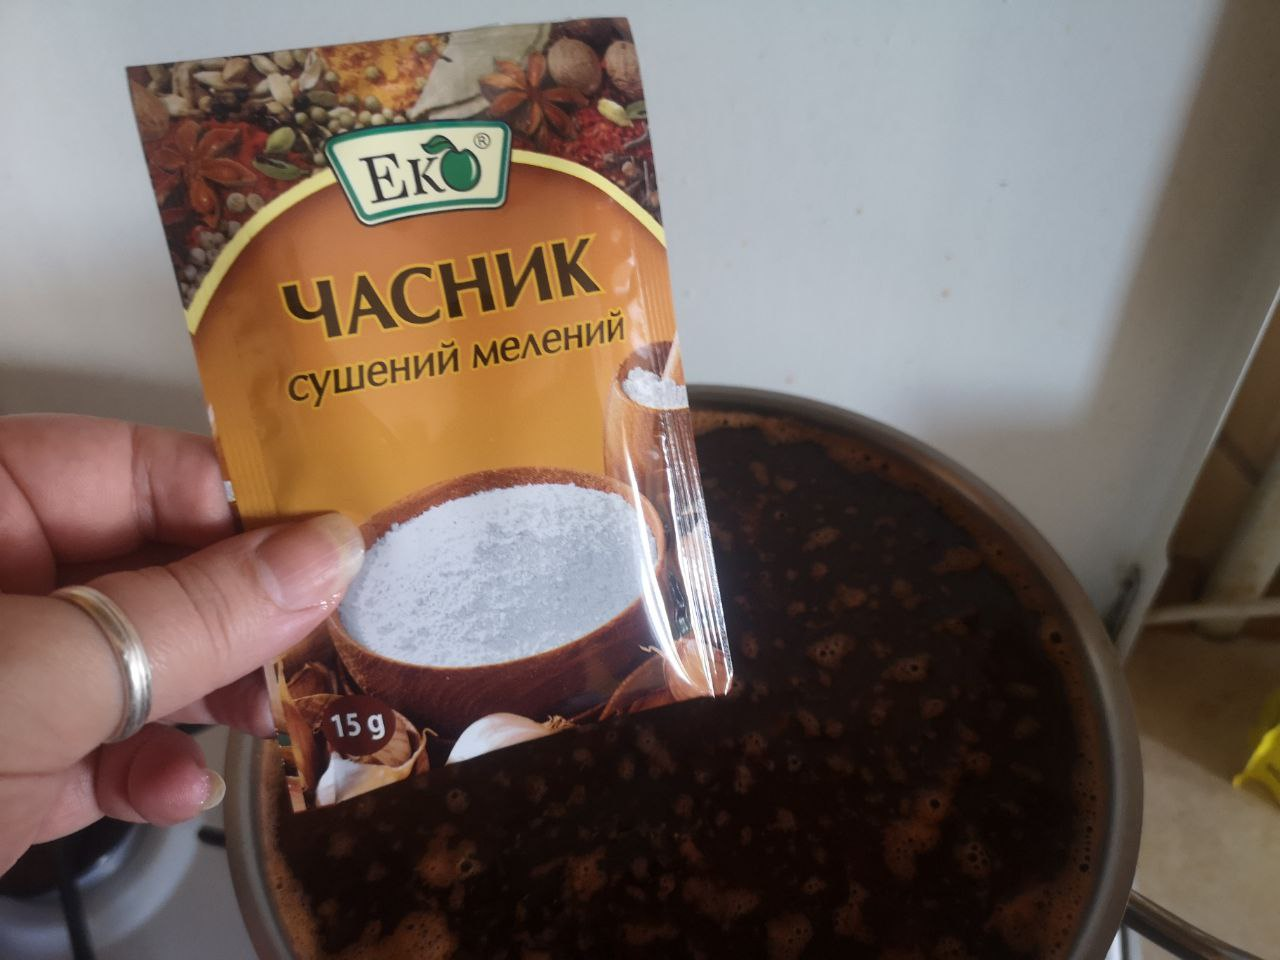
\includegraphics[width=\textwidth]{17.jpg} \\

Let borshch to boil but turn off the stove immediately when it is. \\
Wait at least 15 minutes, add diced green onion to the plate and enjoy: \\
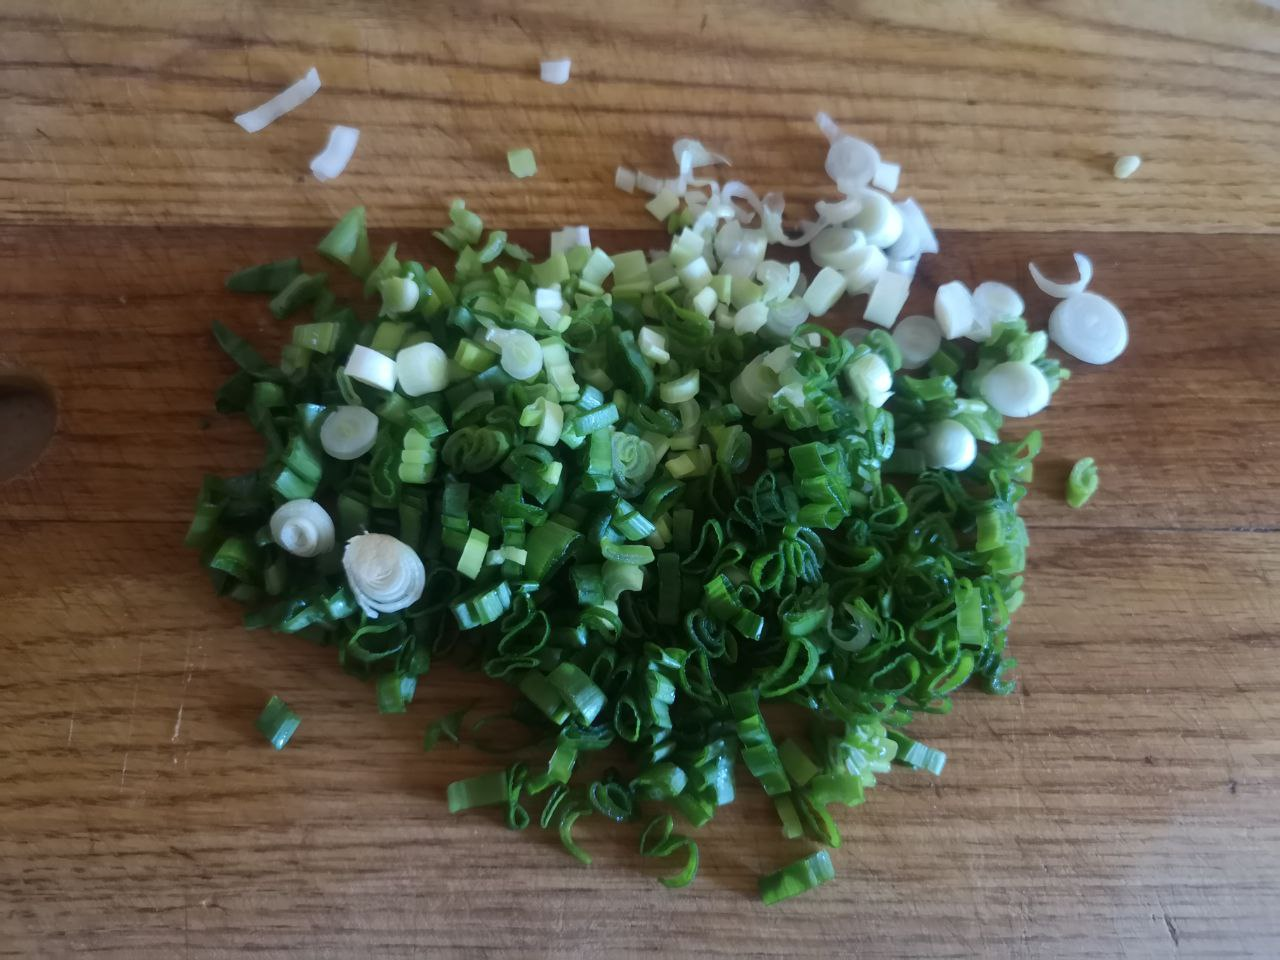
\includegraphics[width=\textwidth]{18.jpg} \\
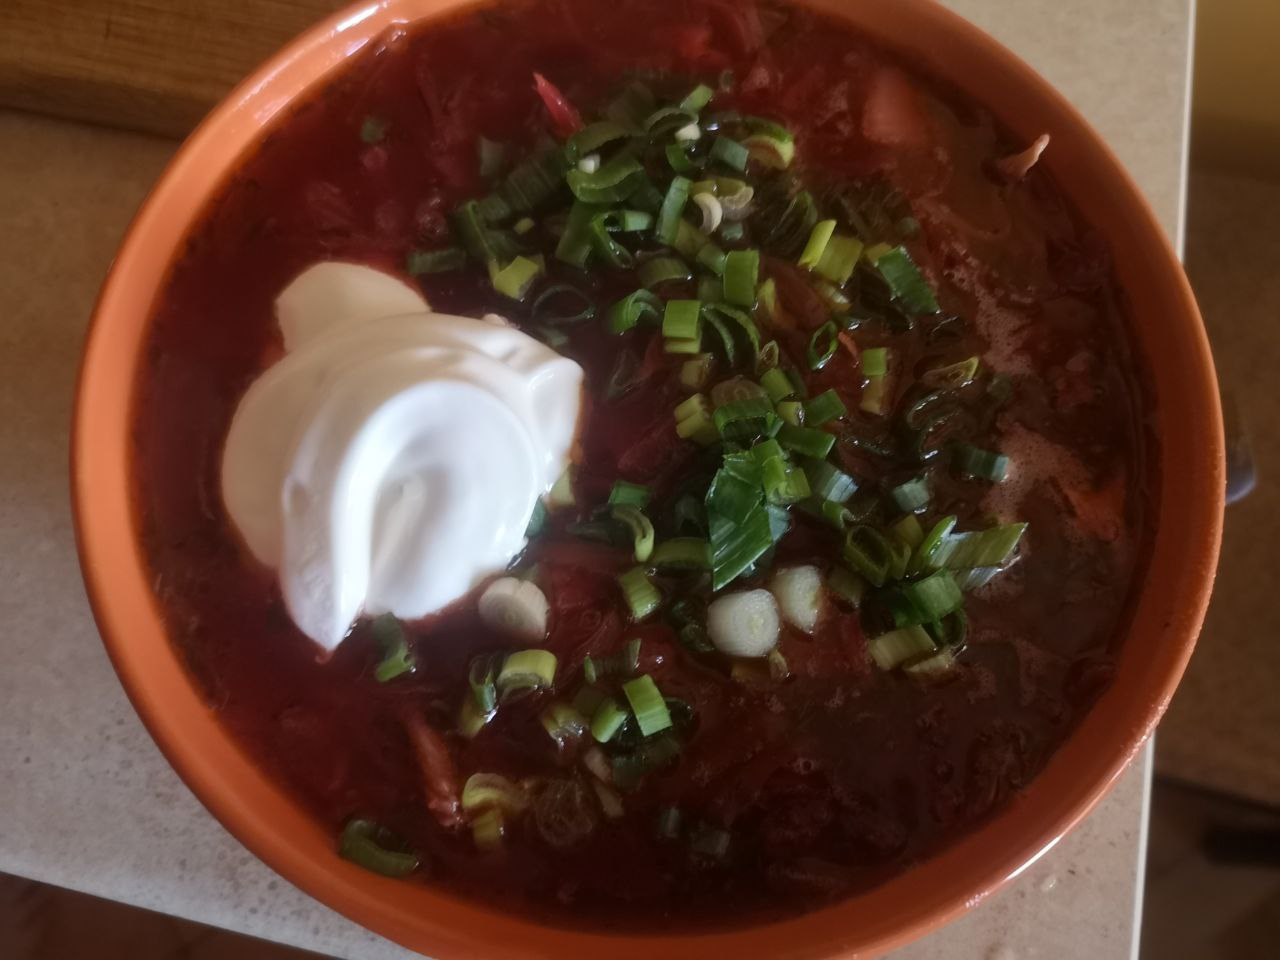
\includegraphics[width=\textwidth]{19.jpg} \\


\section*{Шпундра Shpundra \textipa{['SpundrA]}}
Shpundra is the one of the oldest Ukrainian meals, it was known at least in medieval. The main ingredients are beetroot and meat (originally pork or beef but you can use any other as well). The best way to cook it is using clay pot and oven or cast iron pot on stove but you can use any other pot, even wok. \\
Ingredients:
\begin{itemize}
\item Beetroot
\item Meat
\item Onions
\item Optional: garlic
\item Boiled millet as a side dish
\end{itemize}

Pile and dice meat, beetroot and onion (${\sim}$30x30x30 mm), put them in pot, add salt, pepper and minced garlic, stir well. Usually you don't need to add any water there, onions and beetroot has it a lot. Lid on pot and put it into the oven (180$^{\circ}$ C) or on the stove (low temperature). Let it simmer for 2-3 hours. \\

Before: \\ 
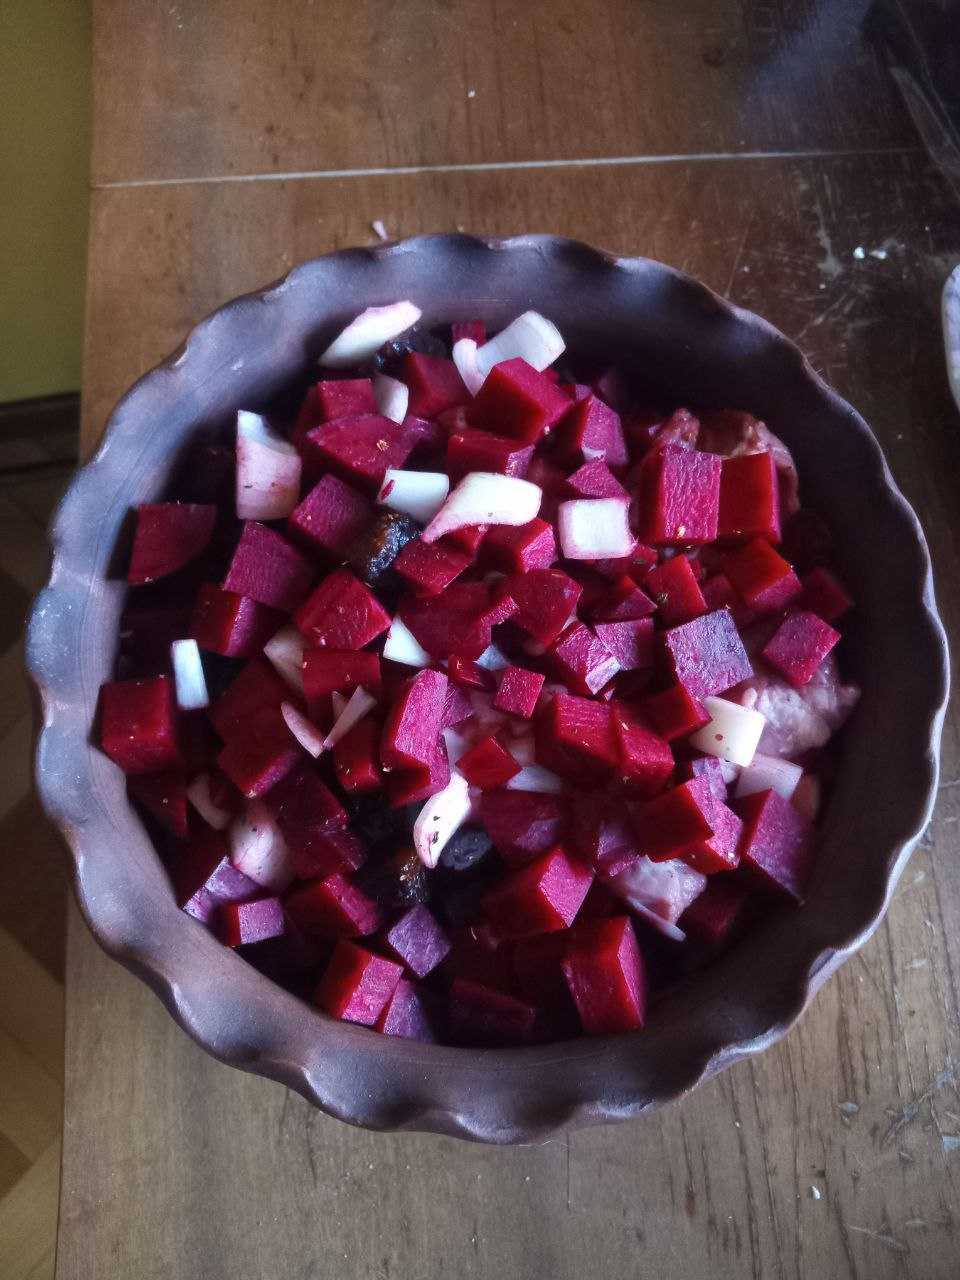
\includegraphics[scale=0.25]{shpundra_1.jpg} \\

After: \\
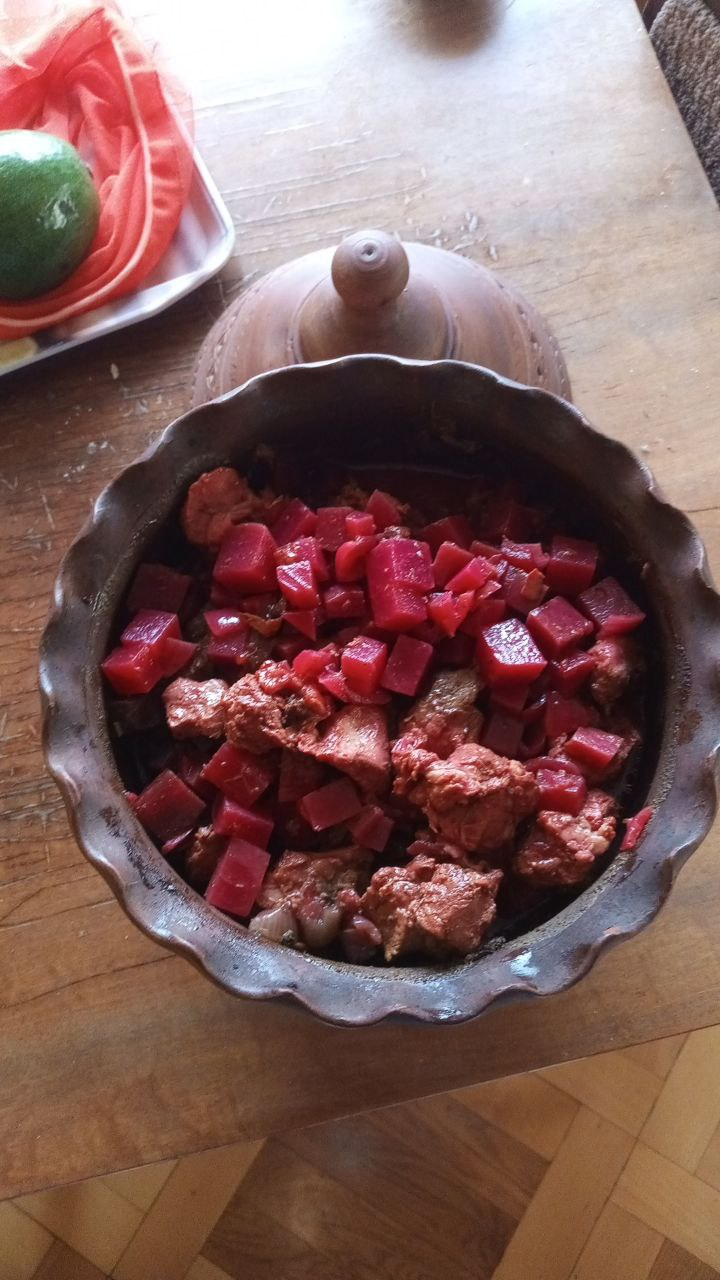
\includegraphics[scale=0.25]{shpundra_3.jpg}

Before shpundra became ready boil millet as usual (millet and beetroot has awesome tastes combination).


\newpage
\
\newpage
\doclicenseThis

\end{document}	